% Source: https://tex.stackexchange.com/a/209658
\documentclass[tikz]{standalone}
\usepackage{pgfplots}
\pgfplotsset{compat=1.7}
\begin{document}
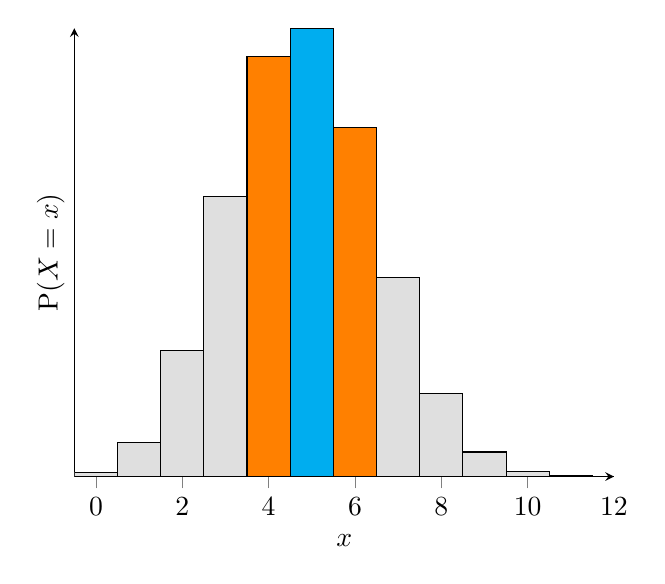
\begin{tikzpicture}[
    declare function={binom(\k,\n,\p)=\n!/(\k!*(\n-\k)!)*\p^\k*(1-\p)^(\n-\k);}
]
\begin{axis}[ymin=0, xmin=-0.5,axis lines=left,xlabel={\(x\)}, ylabel={\(\mathrm{P}(X=x)\)}, 
    samples at={0,...,12},
    yticklabel style={
        /pgf/number format/fixed,
        /pgf/number format/fixed zerofill,
        /pgf/number format/precision=2
    },
    ybar=0pt, bar width=1, bar shift=0pt,
    ymajorticks=false,
]
\addplot [fill=gray!25] {binom(x,12,0.4)}; 
\addplot [fill=orange, samples at={4,6}] {binom(x,12,0.4)};
\addplot [fill=cyan, samples at={5}] {binom(x,12,0.4)};
\end{axis}
\end{tikzpicture}
\end{document}